\section{Выполнение работы в microcap}
Для диода \texttt{D2d2998d}, я выполнил моделирование лабораторного стенда в программе \textbf{Microap} для получения его ВАХ как на прямой цепи, так и на обратной.
\begin{figure}[H]
	\centering
	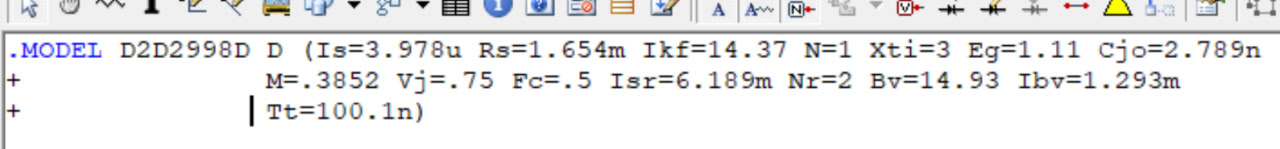
\includegraphics[width=1\textwidth]{img/02.jpg}
	\captionsetup{font=footnotesize}
	\caption{Характеристики моего диода. Вар по списку: 16. Вари диода: 148}
	\label{fig:02}
\end{figure}

При обратном смещении диод ведёт себя как переменная ёмкость, величина которой зависит от приложенного напряжения. Для определения этой ёмкости можно использовать косвенный метод, измеряя резонансную частоту контура с подключённым диодом. Для этого можно собрать следующую схему, которая позволит измерить резонансную частоту.
\begin{figure}[H]
	\centering
	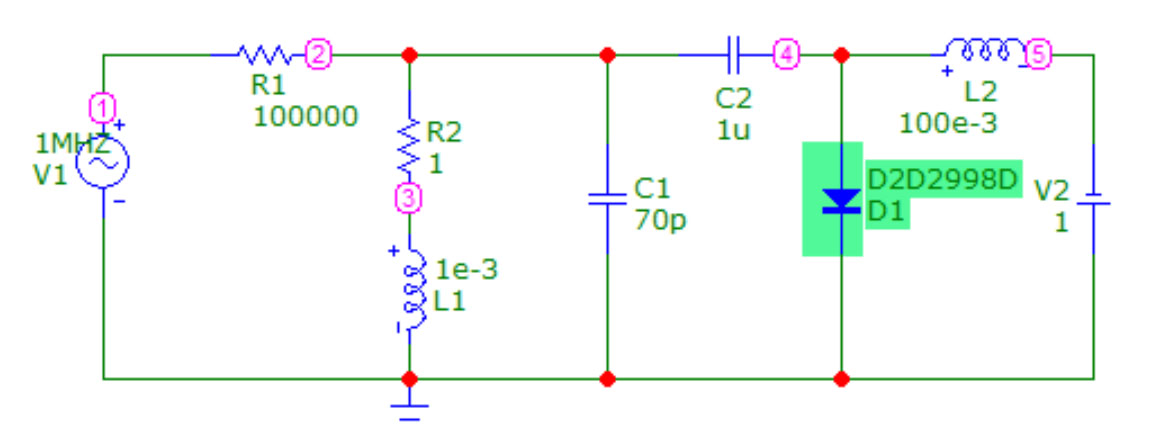
\includegraphics[width=1\textwidth]{img/01.jpg}
	\captionsetup{font=footnotesize}
	\caption{Схема для исследования}
	\label{fig:01}
\end{figure}

\newpage

Резонансную частоту параллельного колебательного контура можно предварительно рассчитать с помощью формулы Томпсона:
\begin{figure}[H]
	\centering
	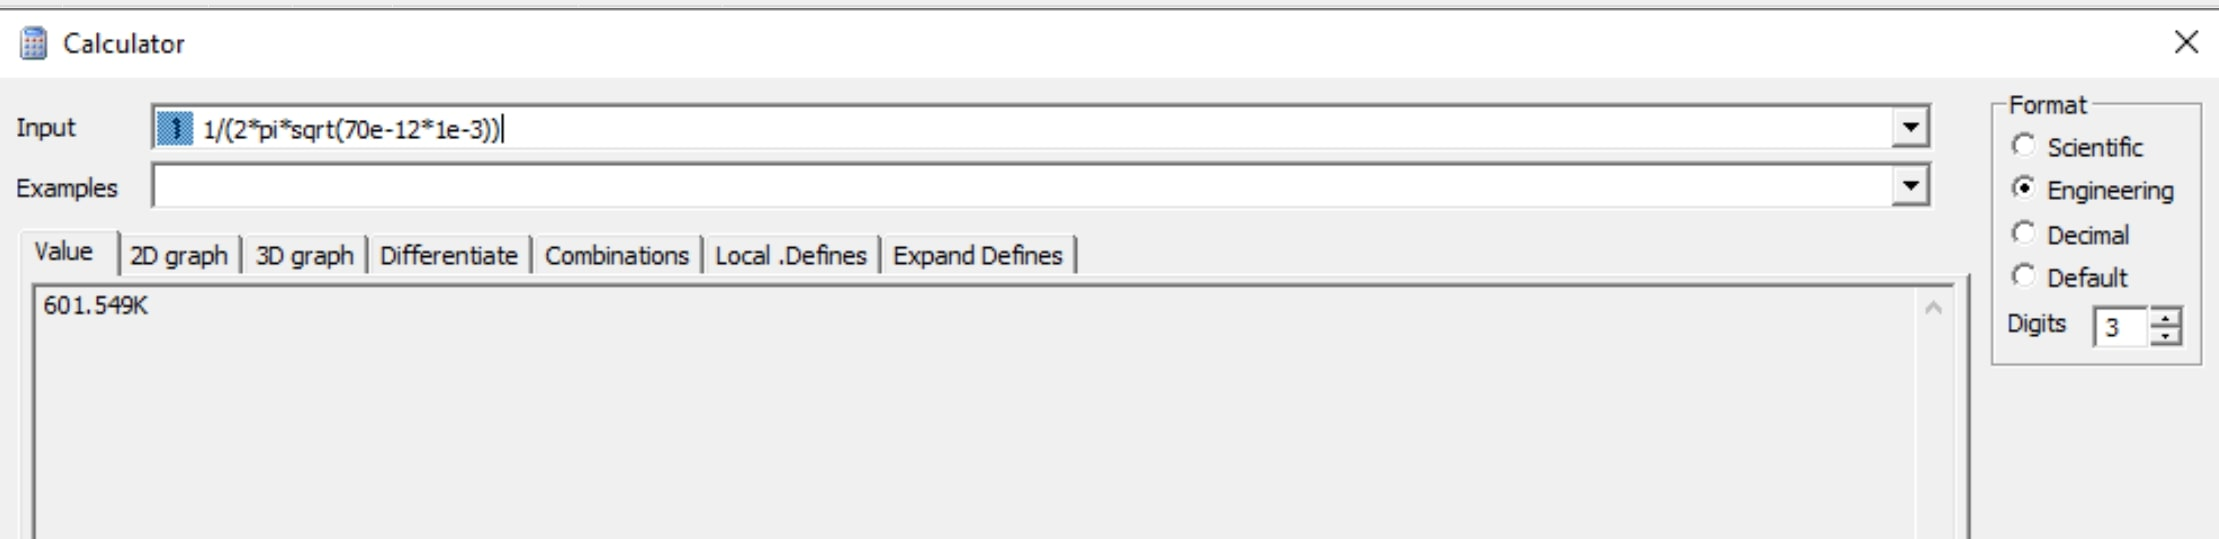
\includegraphics[width=1\textwidth]{img/03.jpg}
	\captionsetup{font=footnotesize}
	\caption{Частота контура}
	\label{fig:03}
\end{figure}

Затем я подключил диод параллельно к схеме и экспериментально определил резонансную частоту нового контура при различных значениях напряжения \texttt{V}. Для этого проводим анализ переменного тока \textbf{AC analysis}, задавая диапазон частот от $200$ кГц до $600$ кГц. Этот диапазон выбран на основе формулы Томпсона, которая показывает, что частота колебаний контура без диода составляет $600$ кГц, а подключение диода снизит эту частоту.
\begin{figure}[H]
	\centering
	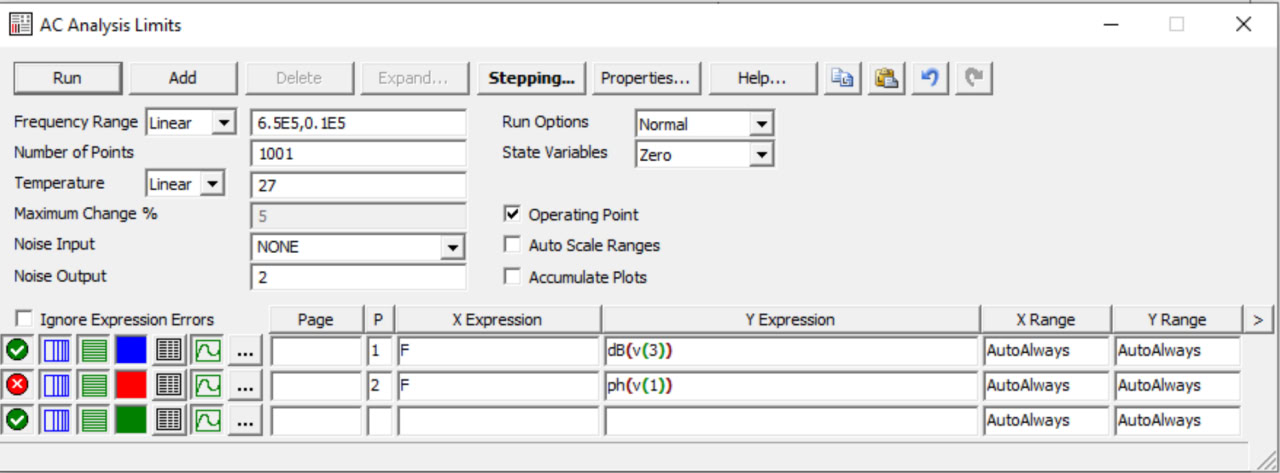
\includegraphics[width=1\textwidth]{img/04.jpg}
	\captionsetup{font=footnotesize}
	\caption{Диапазон значений переменного тока}
	\label{fig:04}
\end{figure}

\begin{figure}[H]
	\centering
	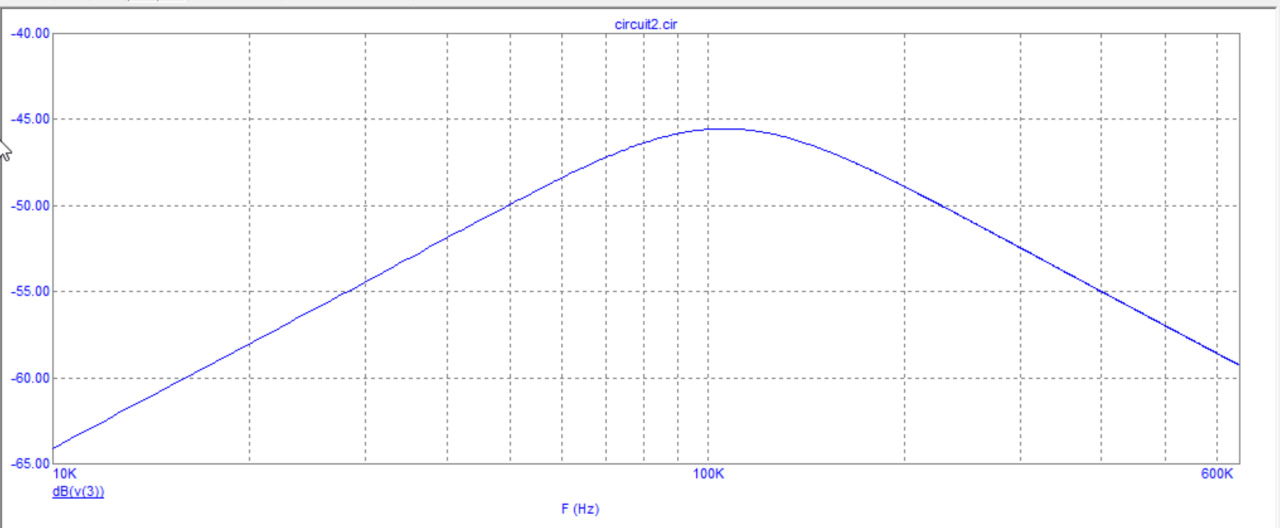
\includegraphics[width=1\textwidth]{img/05.jpg}
	\captionsetup{font=footnotesize}
	\caption{Резонансная кривая}
	\label{fig:05}
\end{figure}


Устанавливая различные значения напряжения на источнике управления \texttt{V2}, можно зафиксировать зависимость резонансной частоты от этого напряжения. Для этого включаем многовариантный режим анализа, используя функцию \textbf{Stepping}, и выполняем анализ для напряжений от $1$ до $10$ вольт с шагом $1$ вольт.
\begin{figure}[H]
	\centering
	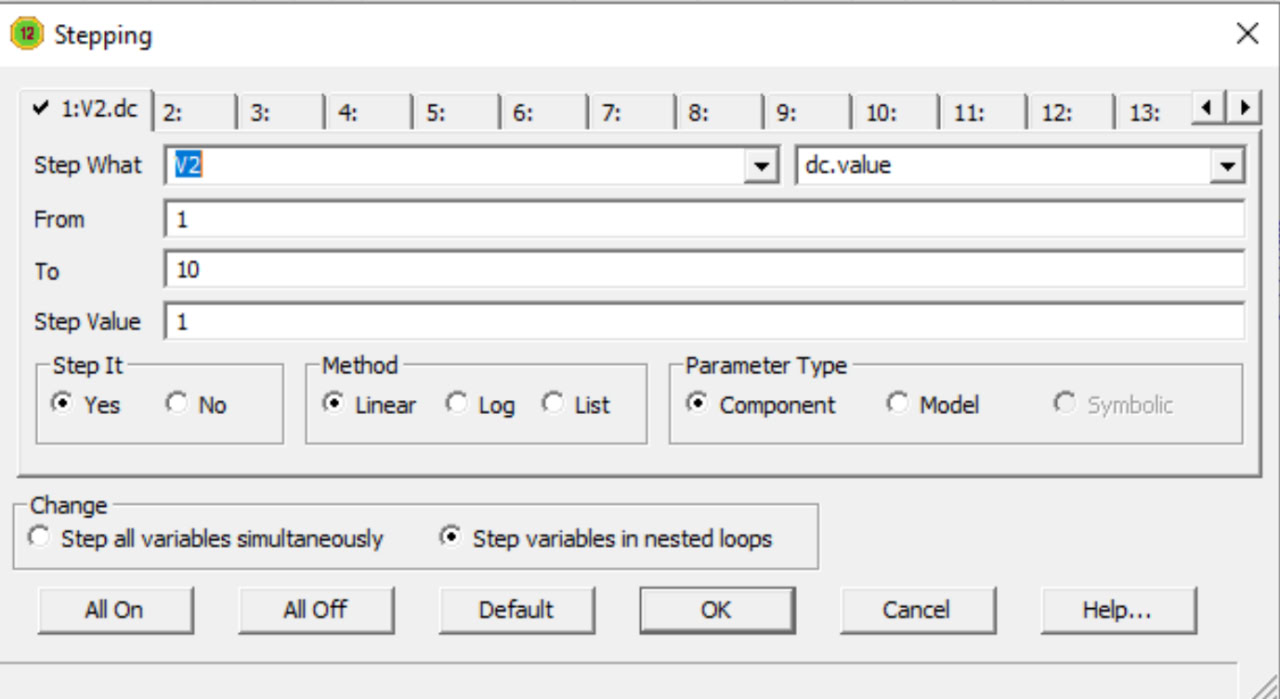
\includegraphics[width=1\textwidth]{img/06.jpg}
	\captionsetup{font=footnotesize}
	\caption{Конфигурация Stepping}
	\label{fig:06}
\end{figure}

\begin{figure}[H]
	\centering
	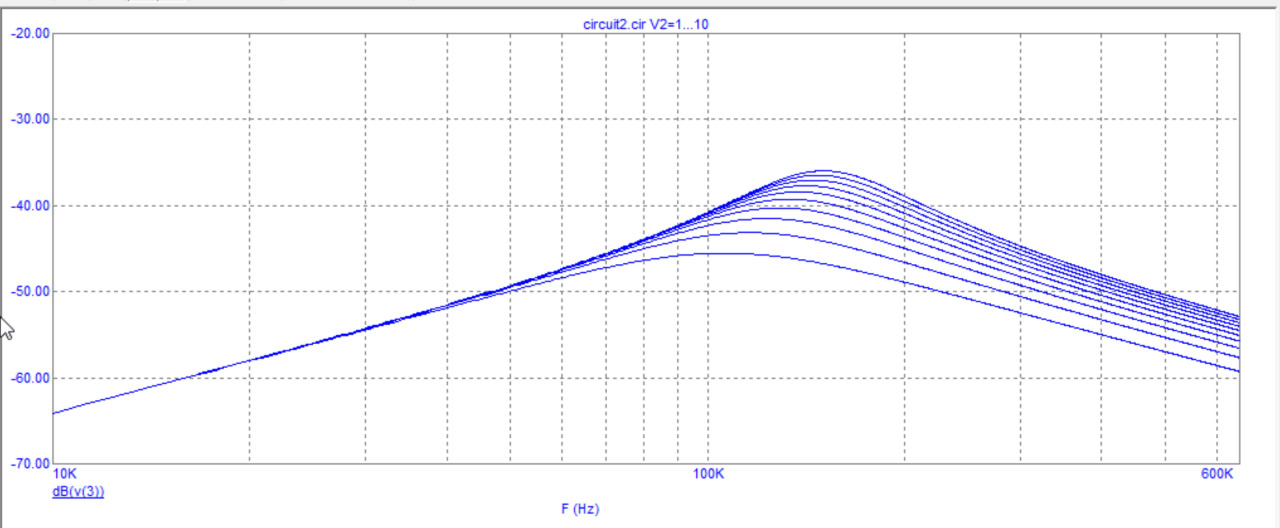
\includegraphics[width=1\textwidth]{img/07.jpg}
	\captionsetup{font=footnotesize}
	\caption{Резонансные кривые в зависимости от смещения на диоде}
	\label{fig:07}
\end{figure}
Исходя из графиков, можно отметить резонансные частоты, а именно точки
максимума, при различных уровнях напряжения.


